\chapter{Methods}
\label{ch:Methods}

The purpose of this chapter is to based on the theory given in the previous chapter present an extended VAHSS construction that ensures honest clients by verifying that their inputs is from an allowed range or set. This will be done by first evaluating the performance of the range proofs discussed above to get an understanding of their advantages and disadvantages.This will be used to then determine which are more suitable to use in a extended VAHSS construction.. In the section \ref{sec:combination} details on how to construct a VAHSS scheme that ensures honest clients is derived. The next section investigates the possibility of  improving of the combined construction by aggregating the  clients individual range proofs into one combined range proof. Then the final section discuss details about how to implement the construction presented in section \ref{sec:combination} is discussed. 

\section{Comparison of constructions for verify clients honesty}
In this section the different constructions for verifying clients honesty presented in section \ref{sec:RF_theory} will be compared to obtain an understanding of their suitability to be combined with the VAHSS scheme described in Construction \ref{alg:VAHSS-HSS} to verify clients honesty. The aspects that  is of interest in the evaluation of the range proofs and their compatibility with the VAHSS construction is presented is the below list;
\begin{itemize}
    \item Computation complexity  (for setup, prover verifier)
    \item Proof size (communication complexity)
    \item Flexibility of range
\end{itemize}

Remark that all of the range proof considered aim to prove that the secret in a Pedersen commitment is in an allowed range (or set). Thus to combine any of the range proofs with the VAHSS construction, the clients needs to publish a Pedersen commitment of their secret $x_i$. This is investigated further in section \ref{sec:combination} and it will be shown that the adaptation of the VAHSS construction to include a range proof is the same independent of the range proof used, hence the adaptability to VAHSS in not considers in the evaluation.

%The considerable difference between the Bulletproof and the signature based range proofs makes the comparison between them not straightforward.  Signature based range proofs requires bilinear mappings unlike Bulletproofs, bilinear mappings are relative expensive operation compared to for example group exponentials which are dominating  the computational complexity for Bulletproofs. Therefore it is not straightforward to compare them in aspects of number of operations performed and an explicit comparison will only be made with respect to runtime. But first the theoretical performance  and properties of the range proofs will be discussed individually.

A small first analysis is that the verification time of the range proofs and set membership proofs will become mostly important when used in a VAHSS construction, this is since there are usually many clients participating and thus the verification will, without aggregation as discussed later, grow linear with the number of clients. This  is further discussed later in section \ref{sec:aggregation}.


\subsection{Theoretical analysis}
The computational complexity will not be compared theoretically since the Bulletproofs is considerable different in the construction compared to the set membership proof and signature based range proof. The latter requires bilinear mappings unlike Bulletproofs, bilinear mappings are relative expensive operation compared to for example group exponentials which are dominating  the computational complexity for Bulletproofs. Therefore instead of comparing the theoretical computational complexity the runtime for prototype implementation of the different proof is considered in the next section. 

However here the communicational complexity for the set up phase for the set membership proof will be discusses. The set membership proof requires $n=|\Phi|$ digital signatures to be known by both prover and verifier, one signature for each elements in $\Phi$. This signatures are usually shared by the verifier in the Setup phase. Sharing the digital signatures of the elements in the set $\Phi$ becomes intractable when the set is large.  If it can be assumed that these signatures has been pre shared, for example in application where the same set of signatures are used many times, then the set membership can still be competitive to range proofs for applications requiring large sets. Large here refers to sets of size $>100$. 

The communicational complexity of the proofs is not the most important feature of comparison, but it is still an important factor and hence the proof size  is briefly discussed  for the different proofs. Given that the digital signatures are pre-shared the set membership provides a $\mathcal{O}(1)$-size set membership proof. The proof size for the signature based range proof is $\mathcal{O}\big(\frac{k}{log\: k- log\:log\:k}\big)$, where $l = \frac{k}{log\: u}, u = \frac{k}{log\: k}$ and for Bulletproofs $\mathcal{O}(log_2n)$. Thus it can be realised that the proof size for set membership is theoretically smallest and signature based range proofs largest. 

A big advantage of the set membership is that it allows to prove that a secret belongs to a set instead of a range and this is much more general. For example a set can be all prime numbers from $1-1000$, all odd numbers or just a random set of numbers. While the signature-based range proof and Bulletproof can only be use to prove belonging to a continuous range. In the paper presenting signature-based range proof is seen that a secret can be proven to belong to arbitrary ranges $[a,b]$ ,where that $a>0$ and $b>a$, and not only ranges where the lower bound is $0$. Considering arbitrary boundaries leads to a doubling of the computational complexity and communication complexity. Actually Bulletproofs can be modified to also allow arbitrary range, $[a,b]$, with a similar approach as presented for the signature based range proofs and illustrated in Figure \ref{fig:interval}. A Bulletproof where one prover wishes to verify the range of several commitments can be optimised such that the  proof size does not growing multiplicatively in the number of commits but instead grows additive. More precisely lets a assume a prover wants to prove the range of $k$ commits a naive implementation would lead to a proof size of $k\cdot log_2 n $, but an optimised implementation reduces this to $log_2 n + 2 log_2 k$.  Hence for the case of arbitrary intervals  proof size is increased with the additive term $2log_2 2 = 2$. The computational complexity grows.. TODO %
Both for  signature-based range proof  and Bulletproof it is not the actual interval that a secret is proved to belong to ($[a,b]$) that determines the complexity, it is the size of $u^l$ respective $2^n$ in the constructions. This is seen by how the bounds $a,b$ are just used for rewriting the secret and does not accurately affect the construction.
It is required that $b< u^l$ for the signature based range proof and $b<2^n$ for the Bulletproofs. Thus the complexity is not dependent on the size of the range but rather the upper limit, this leads to that even a small range of large numbers results in longer runtime. Set membership proofs does not have this property since the runtime for the proof construction and verification is independent of the size and values of the elements in the set. Concluding set membership proof allows proving belonging to much more flexible sets than the range proofs, but both range proofs considered can prove belonging to ranges $[a,b]$, where $a>0$ and $b>a$. 

\begin{comment}
\subsection{Theoretical analysis: Signature-based set membership and range proof}
First lets discuss the communication complexity and proof size starting with the signature based set membership . This construction allows for a $\mathcal{O}(1)$- size proof that a committed value belongs to a given set $\Phi$. In order to construct such a proof $n=|\Phi|$ digital signatures needs to be known by both prover and verifier, one signature for each elements in $\Phi$. This signatures are usually shared by the verifier in the Setup phase. Sharing the digital signatures of the elements in the set $\Phi$ becomes intractable when the set is large.  A large set in this context would be a set consisting of a few hundred elements since the verifier has to publish $n$ digital signatures in the SetUp phase. 

The signature based range proof reduces this to only needing to publish $u$ digital signatures to prove a commitment is in the range $[0,u^l]$ in the SetUp phase. In the algorithm \textbf{Prove} in Construction \ref{alg:ZKRP} the prover sends $l+1$ elements from the group $\mathds{G}_1$, $l$ elements from the group $\mathds{G}_T$ and $2l+1$ field elements. Comparing to the algorithm \textbf{Prove} in Construction \ref{alg:ZKSM} where the prover sends two elements from the group $\mathds{G}_1$, one elements from the group $\mathds{G}_T$ and three field elements. For the ZKRP the communication complexity depends on the choice of $u,l$. Asymptotic analysis gives a communication complexity $\mathcal{O}(\frac{k}{log\:k-log\:log\:k})$, where $l=\frac{k}{log\:u}$ and $u$ put to $u=\frac{k}{log\: k}$ Here $k$ satisfies $u^l \geq 2^{k-1}$.

For ZKSM the communicational complexity for the proof is lower then for the ZKRP, given $l>1$. In some practical applications the digital signatures shared in the setup phase can be assumed to be pre shared, for example in applications where $\Phi$ is used many times. This leads that ZKSM is to prefer over ZKRP in such applications or when $\Phi$ is a relative small. 

Next consider the computational complexity for algorithms \textbf{Prove} and \textbf{Verify} in the ZKSM and ZKRP. constructions  In the set membership construction both the prover and verifier has to perform one bilinear paring and two exponentials over the group $\mathds{G}$. While in the range proof construction the prover need to perform $l$ bilinear mappings and $5l$ exponentials to prove a secret is in the range $[0,u^l)$ and additionally $3l$ exponentials for arbitrary ranges $[a,b]$. The verifier need to ?? Discuss on meeting.
 %TODO
An advantage of the set membership construction is that it can prove membership of non continuous sets. An example could be that the set $\Phi$ represents all odd numbers in a certain interval and then the prover can insure the verifier that the secret is an odd number in a given range. This is an illustrative example of the flexibility of set membership proofs compared to range proofs.

\subsection{Theoretical analysis: Bulletproof}
First the communication and computational complexity of the inner product argument which is used in the Bulletproof is considered. Then based on this the Bulletproofs will be analysed.

The inner product argument as described in Construction \ref{alg:inner_product}, compared to the naive approach, reduces the communication complexity for proving the statement in equation \eqref{eq:IPA} from linear to logarithmic size in terms of the vecotrs length.  More precisely the prover has to send $2\lceil log_2 n \rceil$ group elements and $2$ field elements to the verifier when proving the statement, thus the commutation complexity id of order $\mathcal{O}(log_2 n)$, where $n$ is the length of the vectors. 

The computational effort for the inner product argument is dominated by $8n$ group exponentiations for the prover and  $4n$ group exponentiations for the  verifier. In a non-interactive construction this can be optimised such that the verifier instead perform only one multidimensional-exponent of size $2n+ 2log_2n +1$. This leads to a significant speed up of the verification of the argument.     

Using the inner product argument to build Bulletproofs result in a communication complexity of $2\lceil log_2 n \rceil +4$ group elements and $5$ field elements, where $n$ is such that a secret is proved to be in the range $[0,2^n)$.  A remark is that in a Bulletproof construction the range always has to be an exponent on $2$, if the length of the binary representation of the secret is not a two-exponent this can be solved with padding. When extending the Bulletproof to prove a secret is in an arbitrary range $[a,b]$ the communication complexity is increased by an additive term of size $2$.  

\end{comment}
\subsection{Prototype Analysis}
\label{sec:PrototypeAnalysis}
Implementation of Bulletproofs and signature-based range proof has been done  and compared between them self in \cite{RANGE-SET}, this comparison does not include results about the runtime for the set membership proof. In order to obtain a fair comparison between Bulletproofs, signature-based range proofs and set membership proofs the code used by \cite{RANGE-SET} is benchmarked for all three constructions. The reason for redoing the benchmarking for Bulletproof and signature based range proofs is since else the hardware differences would not lead to a fair comparison. Table \ref{tab:runtime} shows the time complexity comparison between Bulletproofs and signature-based range proofs and set membership proofs implemented in Golang (Go) with $128$- bit security level.  The settings for the benchmarking is the same as in \cite{RANGE-SET}  and the code \cite{Git:RP} except the hardware. The set used in the set membership contain $182$ elements, which thereby is the same amount of elements in the set as length of the range, which is $[18,200]$, for the two range proofs 
% The comparison made by \cite{RANGE-SET} does not does not include results about the runtime for the set membership proof. The runtime for set membership proof included in Table \ref{tab:runtime} is obtained by the author of this paper by benchmarking the code found at \cite{Git:RP}. The settings used are the same as used to obtain the time complexity for the other two range proofs except the hardware parameters.
The computer used has a $1.6$ GHz Dual-Core Intel Core i$5-5250$U CPU, $8$GB $1600$ MHz DDR3 RAM  and running macOS $10.15$. 



%TODO test again
\begin{table}
	\centering
	\caption{Time Complexity comparison for range proof, values are computed as described in section \ref{sec:PrototypeAnalysis}. The runtime are for implementations written in Golang and the implementations are not guaranteed to be optimized in runtime. }
	\label{tab:runtime}
	\begin{tabular}[t]{ l c c }
			 \toprule
    									 		&Generate Proof (ms)	&		Verification  (ms)\\ \midrule		
  			Bulletproof   				&   $ 198$   & $ 79$ 	\\
    			Signature-based 		&   $ 240 $   				&	$438$  \\
    			Set Membership 		&		$66$				&	$90$	\\
			\bottomrule		
	\end{tabular}
 \end{table}

 In Table \ref{tab:runtime} it is clear that the signature based range proof is much slower then Bulletproofs, especially  in the verification. The runtime for verifying the proofs is most important for applications with multiple clients since a verifier has to verify all clients. The runtime for verification between Bulletproofs and Set memberships proofs are rather similar, although Bulletproofs are somewhat faster, which as mentioned is of importance in applications with many clients. 
	
\section{Additive homomorphic secret sharing with verification of both clients and severs }
\label{sec:combination}

The  VAHSS constructions  discussed in section \ref{sec:VAHSS} assumes honest clients and verifiers that the servers computations are correct. The aim of this paper is to extended this VAHSS construction to verify both client and servers. The clients does however not which to reveal their secrets.  A method for verifying clients honesty is zero-knowledge range proof or set membership proofs. If such a proof was included in the VAHSS construction then, under the assumption that there exist an allowed rang or set to which the input must belong, a potentially malicious client can only have limited influence on the computed sum. This is due to that a malicious input must still belong to the allowed range or set and hence the impact on the sum is bounded by the size of the range or the elements in the set. 

Next the combining of range proofs and the VAHSS construction will be discussed, it is not sufficient to construct and perform a range proof and VAHSS  scheme separately, since then the verifier cannot be sure that the secret proven to be in the allowed range is the same as the secret hidden by the shares. Remark that all considered range proofs emanate from a Pedersen commitment hiding a secret and generates a zero knowledge proof that this secret belongs to an pre-specified interval or set. Besides this common feature the range proofs construction differ considerably. Hence the possibility to exploit the Pedersen commitment to link the VAHSS construction with a range proof is investigated, more precisely a link between the shares hiding the secret generated in the algorithm \textbf{ShareSecret} in the VAHSS construction and the secret hidden in the  Pedersen commitment used in the range proof is desired to convince the verifier that the shares represents a secret that is in the allowed range.  As mentioned publishing a Pedersen commitment of the secret itself does not provide any guarantee that it is the same secret that is hidden in shares. Committing to the shares in the Pedersen commitment is neither an option, the individual shares themselves does not reveal information about the secret they are hiding. This leads to that there is not guarantee that proving a share belongs to the allowed range (or set) implies that the secret does and the other way assuming that the secret to a range (or set) does not imply that the shares does. Thus some trick to connect the secret in the shares to the secret in the Pedersen commitment must be derived. The aggregation used in the VAHSS construction to prove the honesty of the servers is tested if it can also be used to also connect the range proofs to the VAHSS construction.

Recall that the clients except from the shares also publishes the checksum $\tau_i$ for the secret $x_i$, more precisely the definition of the checksum is  $\tau_i=g^{x_i+R_i}$, where $R_i$ chosen uniformly at random. This checksum is indeed equal to a Pedersen commitment where $g=h$. Using this checksum as the Pedersen commitment in the constructing of a range proof would be sound. However if $g=h$ the computationally biding property of a Pedersen commitment would not hold since $log_g(h)=log_g(g)=1$ which leads to that the left hand side in equation \eqref{eq:pedersen_binidng} is equal to $1$. Therefore to construct two commits $\mathds{E}(x,R)$ and $\mathds{E}(x',R')$ such that $\mathds{E}(x,R) = \mathds{E}(x',R')$ but $x\neq x'$ it is sufficient to solve solve $x'$ in, 
\begin{align*}
1 = \frac{x-x'}{R-R'}\:mod \:N.
\end{align*}
In other words it is straightforward to create a false commitment hence also a false range proof. Lets instead investigate modifying the checksum $\tau_i$ to a Pedersen commitment. Let the clients compute and output $\pi_i=g^{x_i}h^{R_i}$, where $x_i,R_i,g,h$ are as defined above, instead of $\tau_i$ as before.  Now a range proof can easily be constructed for the commitment $\pi_i$. Below it will be shown that Theorem \ref{thm:VAHSS_CSV} still hold after replacing $\tau_i$ with $\pi_i$. It remains to argue that this method ensures the verifier that the secret hidden by the shares is the same secret proven to be in the allowed range by the range proof. 

Assume that client $k$ commits to the value $\hat{x}_k$ in the Pedersen commitment $\pi_k$ and generates a range proof that the secret hidden in the commitment belongs to the interval $[a,b]$ but constructs shares $\{x_{kj}\}_{j=1}^m$ such that $\sum_{j=1}^m x_{kj} = x_k \neq \hat{x}_k$. Then when verification of the servers honest it will not hold that $\prod_{i=1}^m \pi_i = g^y$. Therefore the verification will return false and the protocol will not succeed even if the range proof does. Although any cheating party will be detected, it will not be possible do determined which party that cheated more precisely not even if the cheating party was a client or a server. 

In Construction \ref{alg:VAHSS-HSS-RP} the extended VAHSS is described in detail. In order to clarify the modifications made to include a range proof, lets briefly mention some differences to the VAHSS construction presented in \cite{SumItUp} ans also presented in Construction \ref{alg:VAHSS-HSS}. The algorithms \textbf{ShareSecret} and \textbf{Verify} has been modified,  and the algorithms \textbf{RangeProof} and \textbf{GenerateCommitment} have been added. More precisely in the algorithm \textbf{ShareSecret} does not output the checksum $\tau_i$, instead the Pedersen commitment $\pi_i$ is computed in the algorithm \textbf{GenerateCommitment}, this algorithm can be included in either \textbf{ShareSecret}  or \textbf{RangeProof} instead of being viewed as a separate algorithm, in the implementation discussed below the commitment is generated while constructing the range proof and not explicitly. The algorithm \textbf{RangeProof} constructs a range proof (or set membership proof) denoted $RP_i$ given the commitment $\pi_i$ and secret $x_i$. Note that it is not specified which range proof construction that is used since it does not affect the rest of construction as long as the verification algorithm used to verify the range proof is the compatible with the construction of the proof. Both algorithms \textbf{ConstructRangeProof} and \textbf{RangeProof} are executed by the clients.. The algorithm \textbf{Verify} additionally to the steps of the algorithm in Construction \ref{alg:VAHSS-HSS} also verifies the correctness of the range proof $RP_i$ and an additional \texttt{AND} operator to compute the total verification. 

%In the VAHSS Construction \ref{alg:VAHSS-HSS} the verifiability property includes verification of the servers. In this section this will be extended to also include the clients. The value $\pi_i$ published by the clients will be modified into a Pedersen commitment on the form $\pi_i = g^{x_i}h^{R_i}$, remember $\pi_i=g^{x_i+R_i}$ in the original construction presented in \cite{SumItUp}. The clients will apart from the previous commitments  also construct and publish a range proof for $\pi_i$. This allows any verifier to apart from verifying the servers also verify that the secret shared by the clients is in an certain range.  

%Given this construction the correctness, security and verification requirements for the server verifiable AHSS presented in \cite{SumItUp} is still fulfilled  that should be fulfilled is redefined below.  The difference to the requirements for the server verifiable AHSS is that additional demands for the clients behaviour is included. 

\begin{comment}
\begin{itemize}
    \item \textbf{Correctness} It must hold that Pr$\Big[\textbf{Verify}(\{\pi_i\}_{i\in\mathcal{N}},\sigma,y,\{RP_i\}_{i\in\mathcal{N}})=1\Big]=1$. This means that 					with probability $1$ the output $y$ from \textbf{FinalEval} is accepted given all parties (clients and servers) where honest and the protocol were executed correctly.
    \item \textbf{Security} 
    			\begin{itemize}
    						\item \textbf{Malicious Servers } The construction should satisfy the same security argument as the VAHSS-HSS construction in \cite{SumItUp}.
    						%Let $T$ define the set of corrupted servers such that $|T|<m$, i.e at 					least one server is honest.  										Denote a PPT adversary by $\mathcal{A}_1$ and let the Adv$(1^			\lambda,\mathcal{A},T):= \text{Pr}[b' = b]-1/2$ be the advantage 										of $\mathcal{A}=\{\mathcal{A}_1,\mathcal{D}\}$ in guessing $b$ in the following experiment:
    							%		\begin{enumerate}
       						%				 \item The adversary $\mathcal{A}_1$ gives $(i,x_i,x_i')$ to the challenger, where $i\in[n], x_i\neq x_i'$ and $|x_i|=|x_i'|$.
        						%				\item The challenger picks a bit $b\in\{0,1\}$ uniformly at random chooses and computes $\textbf{ShareSecret}(1^\lambda,i,																\hat{x}_i) = (\hat{\text{share}}_{i1},...,\hat{\text{share}}_{im},\tau_i)$, where $\hat{\textbf{x}}_i$ is  such that $\hat{x}_i = 																\begin{cases}x_i, \text{ if } b=0 \\ x_i' \text{ else} \end{cases}$. 
        					%					\item Given the shares from the corrupted servers T and $\hat{\tau}_i$ the adversary distinguisger outputs a guess 																			$b'\xleftarrow[]{}\mathcal{D}((\hat{\text{share}_{ij}})_{j|s_j\in T},\hat{\tau}_i)$.
   									% \end{enumerate}
    							%		A VAHSS-construction is $t$-secure if for all $T\subset \{s_1,...,s_m\}$ with $|T|<t$ it holds that Adv$(1^\lambda,\mathcal{A},T)<												\varepsilon(\lambda)$ for some negligible $\varepsilon(\lambda)$.
  					  \item \textbf{Malicious Clients}  Since the construction does not clarify the exact range proof used, the security argument is refereed to the original papers for the used range proof and by proving that the secret hidden by the Pedersen commitments is the same as the secrets in the shares. 
   		 \end{itemize} 
 	\item \textbf{Verifiability} 
 			\begin{itemize}
 						\item \textbf{Verify Servers }Let $\mathcal{A}$ denote any PPT  adversary and $T$ denote the set of corrupted servers with $T\leq m$. The verifiability 							property requires that any $\mathcal{A}$ who can modify the input shares to all servers $s_j\in T$ can cause a wrong value to be excepted as 							$y=f(x_1,...,x_n)$ with negligible probability.   
 						\item \textbf{Verify Clients} Let $\mathcal{A}$ denote any PPT adversary and $T$ denote the set of corrupted clients. The verifiability property requires that any $\mathcal{A}$ who can modify the Pedersen commitments $\pi_i$  to any $\pi_i^{'} \:\forall  i\in T$ has a negligible probability at choosing a commitment $\pi_i^{'}$ such that Verify$( \{\pi^{'}_i\}_{i\in\mathcal{N}},x,y)=1$.
 			\end{itemize} 
\end{itemize}
\end{comment}

\begin{algorithm}
\caption{\textbf{: Client and Server Verifiable additive homomorphic secret sharing}}

\textbf{Goal:} Construct and share the sum $\sum_{i=1}^n x_i$, where $x_i$ is a secret value known by client $c_i$, where $i\in\mathcal{N}$ without any client needing to revealing their individual secret. All parties are verified to be honest in the construction.
\vspace{2pt}
\hline
\vspace{2pt}
\begin{itemize}
 \item\textbf{ShareSecret $(1^\lambda,i,x_i) \mapsto \{x_{ij}\}_{j\in\mathcal{M}}$} \\
Pick uniformly at random $\{a_i\}_{i\in\{1,..,t\}}\in_R\mathds{F}$ to be the coefficients to a $t$-degree polynomial $p_i$ on the form $p_i(X) = x_i + a_1X+...+a_tX^t$. Define  the shares as $x_{ij}=\lambda_{i,j}p_i(\theta_{ij})$ for $j\in\mathcal{M}$, the parameters $\theta_{ij}$ and Lagrange coefficients $\lambda_{ij}$ is chosen such that equation \ref{eq:pi(0)} is satisfied.
Output $\{x_{ij}\}_{j\in\mathcal{M}}$.

\item\textbf{GenereteCommitment$(1^\lambda,i,x_i) \mapsto \pi_i$ }\\
Let $\mathds{E} : x,y \to g^xh^y$ be a Pedersen commitment . Let $R_i\in\mathds{F}$ be the output of a PRF such that $R_n\in \mathds{F}$  satisfies $R_n = \phi(N)\lceil \frac{\sum_{i=1}^{n-1}R_i}{\phi(N)}\rceil- \sum_{i=1}^{n-1}R_i $. Compute and output $\pi_i = \mathds{E}(x_i,R_i)$.

\item\textbf{RangeProof $(x_i,\pi_i) \mapsto RP_i$}\\
Construct a range proof, denoted $RP_i$, for the commitment $\pi_i$ to the secret $x_i$, on the  range $[0,B]$ ( or a set $\Phi$) using Construction \ref{alg:ZKSM}, \ref{alg:ZKRP} or \ref{alg:bullet}. All required  parameters and setup is assumed to be pre-shared and known by all parties.
\item\textbf{PartialEval $(j,\{x_{ij}\}_{i\in\mathcal{N}})\xrightarrow[]{}y_j$}\\
Compute and output $y_j = \sum_{i=1}^n x_{ij}$.

\item\textbf{PartialProof $(j,\{x_{ij}\}_{i\in\mathcal{N}})\xrightarrow[]{}\sigma_j$}\\
Compute and output $\sigma_j = \prod_{i=1}^n g^{x_{ij}} =  g^{\sum_{i=1}^n x_{ij}}= g^{y_j}=H(y_j)$.

\item\textbf{FinalEval $(\{y_j\}_{j\in\mathcal{M}})\xrightarrow[]{}y$}\\
Compute and output $y = \sum_{j=1}^m y_{j}$.

\item\textbf{FinalProof $(\{\sigma_j\}_{j\in\mathcal{M}})\xrightarrow[]{}\sigma$}\\
Compute and output $\sigma = \prod_{j=1}^m \sigma_j = \prod_{j=1}^m g^{y_{j}} =  g^{\sum_{j=1}^m y_{j}}= g^{y}=H(y)$.

\item\textbf{Verify $(\{\pi_i\}_{i\in\mathcal{N}},x,y,\{RP_i\}_{i\in\mathcal{N}})\xrightarrow[]{}\{0,1\}$}\\
Compute and output $\sigma= \prod_{i=1}^n \pi_i \wedge \prod_{i=1}^n \pi_i = H(y)\wedge \{\textbf{Verify}_{rp}(RP_i)\}_{i\in\mathcal{N}}$. Where $\textbf{Verify}_{rp}$ is the verification algorithm associated with the algorithm used by the clients to construct the range proofs, $\{RP_i\}_{i\in\mathcal{N}}$.
\end{itemize}
\label{alg:VAHSS-HSS-RP}
\end{algorithm}

\begin{thm}
\label{thm:VAHSS_RP_CSV}
\vspace{10pt}
The client and server verifiable AHSS presented in Construction \ref{alg:VAHSS-HSS-RP} satisfies the correctness, security and verifiability requirements described in section \ref{sec:VAHSS}, by replacing $\tau_i$ with $\pi_i$. Additionally it also satisfies the following extension of the verification requirement:

Let $\mathcal{A}$ denote any PPT adversary and $T$ denote the set of corrupted clients. The extended verifiability property requires that any $\mathcal{A}$ who can modify the Pedersen commitments $\pi_i$  to any $\pi_i^{'} \:\forall  i\in T$ has a negligible probability at choosing a commitment $\pi_i^{'}$ such that Verify$( \{\pi^{'}_i\}_{i\in\mathcal{N}},x,y,\{RP_i\}_{i\in\mathcal{N}})=1$.



%\begin{itemize}
 %\item \textbf{Verifiability Servers}  Let $\mathcal{A}$ denote any PPT  adversary and $T$ denote the set of corrupted servers with $T\leq m$. Note that if $|T|=m$, the verifiability property holds but not the security property. The verifiability property requires that any $\mathcal{A}$ who can modify the input shares to all servers $s_j\in T$ can cause a wrong value to be excepted as $y=f(x_1,...,x_n)$ with negligible probability.  
 %\item  \textbf{Verifiability Clients} 
%\end{itemize} 

\end{thm}
%TODO fix proof before hand in to Seminar 2
\begin{proof}
To argue that that the correctness, security and verifiability properties for the server verifiable AHSS still holds after replacing  $\tau_i$ with $\pi_i$ for $i=1,...,n$, it is noted that,
\begin{align*}
&\prod_{i=1}^n \pi_i = \prod_{i=1}^n g^{x_i}h^{R_i} = g^{\sum_{i=1}^n x_i}h^{\sum_{i=1}^n R_i} = g^{\sum_{i=1}^n} h^{ \phi(N)\big\lceil \frac{\sum_{i=1}^{n-1}R_i}{\phi(N) }\big\rceil} = g^y \\
&\text{Hence it follows that: } \prod_{i=1}^n \tau_i = \prod_{i=1}^n \pi_i.
\end{align*}
Further the Pedersen commitment is perfectly hiding and computationally binding and hence it follows that the requirements is still fulfilled. 

It remains to prove that Construction \ref{alg:VAHSS-HSS-RP} also fulfils the extended verification requirement. This follows from the soundness of the range proofs or set membership proof used in the construction and by the argument above that the secret hidden in the commitment $\pi_i$ must be the same as the secret obtain by combining the the shares $\{x_{ij}\}_{j\in\mathcal{M}}$ for all $i=1,...,n$.

\begin{comment}
The correctness follows from the correctness of range proofs and by proving that $\sigma= \prod_{i=1}^n \pi_i \:\bigwedge\: \prod_{i=1}^n \pi_i = \mathcal{H}(y)$. Both $y$ and $\sigma$ are the same as in Construction \ref{alg:VAHSS-HSS}, hence by construction:
\begin{align}
    \label{eq:y=sum(x_ij)}
    y = \sum_{j=1}^m y_j= \sum_{j=1}^m \sum_{i=1}^n \lambda_{ij}p_i(\theta_{ij}) = \sum_{i=1}^n \overbrace{ \Big (\sum_{j=1}^m \lambda_{ij}p_i(\theta_{ij}) \Big)}^{ p_i(0)} = \sum_{i=1}^n p_i(0) = \sum_{i=1}^n x_i,
\end{align}
and for $\sigma$ it holds that:
\begin{align*}
    \sigma = \prod_{j=1}^m \sigma_j = \prod_{j=1}^m g^{y_j} = g^{\sum_{j=1}^my_j} =g^y = \mathcal{H}(y)
\end{align*}
For the $\pi_i$, whose construction has been modified compared to $\tau_i$ in  Construction\ref{alg:VAHSS-HSS}, thus it follows that:
\begin{align*}
    &\prod_{i=1}^n \pi_i = \prod_{i=1}^n \mathds{E}(x_i,R_i)= \prod_{i=1}^n g^{x_i}h^{R_i} = g^{\sum_{i=1}^n x_i } h^{\sum_{i=1}^n R_i} \overset{\eqref{eq:y=sum(x_ij)}}{=} g^y h^{\sum_{i=1}^{n-1} R_i+R_n} = \\ 
    &= g^y h^{ \phi(N)\big\lceil \frac{\sum_{i=1}^{n-1}R_i}{\phi(N) }\big\rceil} = g^y = \mathcal{H}(y) 
\end{align*}

The proof of security argument for malicious servers given in \cite{SumItUp} is still sufficient since the Pedersen commitment is perfectly hiding and computationally binding and that the range proofs are zero knowledge. The security argument for malicious clients follows from the soundness of the range proof and that the secret hidden in the commitment has to be the same as the secret in the shares, as argued above. . 

The proof of \textit{\textbf{Verifiability Severs}} is the same as the proof given in  in \cite{SumItUp}, except that the commitments $\pi_i$ replaces the checksums $\tau_i$.  \textit{\textbf{Verifiability Clients}} follows from the properties of the range proof.
\end{comment}
\end{proof}


\section{Improving runtime}
\label{sec:aggregation}
A desired property for the above presented server and clients verifiable AHSS would be to aggregate the range proofs into one, since then the verifier would have to perform one range proof verification instead of one for each client as in Construction \ref{alg:VAHSS-HSS-RP}. This would decrease the runtime significantly in the verification step, especially in implementations where hundred clients participate. Aggregating the range proofs would require the proofs to be homomorphic, such that the verification remains valid also for an aggregated proof.

A small remark is that the naive approach to aggregate the commitments $\pi_i, \: i\in\mathcal{N}$ to $\pi = \prod_{i=1}^n \pi_i$ and then construct a range proof for the aggregated commitment $\pi = g^{\sum_{i=1}^n x_i}$ over the range $[n\cdot a,n\cdot b]$, to prove $x_i \in [a,b]$ for all $i \in\mathcal{N}$  does not satisfy the verification property in Theorem \ref{thm:VAHSS_RP_CSV}. The value $y=\sum_{i=1}^n x_i$ is publicly known so to construct a zero knowledge range proof for $y $ provides no new information and given that $y\in [n\cdot a,n\cdot b]$ does not imply $x_i\in [a,b]$ for all $i\in\mathcal{N}$. 

\subsection*{Aggregating Set membership proof}
Lets examine the possibility to aggregate the set membership and signature based range proofs, the construction of these two are similar and hence it is sufficient to consider one of them, due to  its simpler notation the set membership proof is considered. Assume two range proofs $RP_1$ and $RP_2$ generated by the algorithm \textbf{Prove} in construction \ref{alg:ZKSM}, recall that such set membership proofs are on the form $RP_i = (V_i,a_i,D_i,z_{x_i},z_{\tau _i},z_{R_i}, )$ for $i=1,2$ and that a proof verifies to $1$ if  $D=C_i^{c_i}h^{z_{R_i}}g^{z_{x_i}}\wedge a_i = e(V_i,y)^ce(V_i,g)^{z_{x_i}}e(g,g)^{z_{\tau_i}}$. In addition to knowledge of the proof the verifier also has knowledge of the commitment $C_i$,  group elements $h,g$  and the challenge $c_i$ can be computed by the verifier. To aggregate the proof each element building the proof would need to be aggregated such that the verification of the aggregated proof can be carried out in the same way as before. First test the straight forward aggregation hence let $RP = (V,a,D,z_{x},z_{\tau },z_{R})$ be the aggregated range proof and  where $V, a, D,z_{x},z_{\tau },z_{R}$ be defined as,
\begin{equation}
\begin{aligned}
\label{eq:naiveAgg}
V =& V_1V_2 = g^{\frac{\tau_1}{\chi + x_1}}g^{\frac{\tau_2}{\chi + x_2}}  = g^{\frac{\tau_1}{\chi + x_1} + \frac{\tau_2}{\chi + x_2}}  \\
a =& a_1a_2 = \big(e(V_1,g)^{-s_1})e(g,g)^{t_1}\big)  \big(e(V_2,g)^{-s_2})e(g,g)^{t_2}\big) \\
=&  \big( e(g,g)^{\frac{-s_1}{\chi+x_1}}e(g,g)^{t_1}\big) \big( e(g,g)^{\frac{-s_2}{\chi+x_2}}e(g,g)^{t_2}\big) \\
D =& D_1D_2 = ( g^{s_1}h^{m_1} ) (g^{s_2} h^{m_2}) = g^{s_1+s_2}h^{m_1+m_2}\\
z_x =& z_{x_1} + z_{x_2} = (s_1-c_1x_1)+(s_2-c_2x_2)\\
z_R =& z_{R_1} + z_{R_2} = (m_1-c_1R_1)+(m_2-c_2R_2)\\
z_\tau =& z_{x_1} + z_{x_2} = (t_1-c_1\tau_1)+(t_2-c_2\tau_2)\\ 
\end{aligned} 
\end{equation}
%are the multiplication of the corresponding elements in the two non aggregated range proofs and are the addition of the corresponding elements in the two non aggregated range proofs. To clarify two examples are, $D=D_1*D_2 =g^{s_1}h^{m_1}*g^{s_2}h^{m_2} = g^{s_1+s_2}h^{m_1+m_2}$, and the two exponentials are now refereed to as $s,m$, more over $z_x = z_{x_1}+z_{x_2} = (s_1-x_1c_1 )+ (s_2-x_2c_2) = s- x_1c_1-x_2c_2 $.
Further also calculate the challenges $c_1$ and $c_2$ according to $c_i=Hash(a_i,D_i),\: i=1,2$ and remember that the  commitments $C_i$  are homomorphic, which follows directly from the homomorphic properties of the Pedersen commitment. It is less obvious to see that the bilinear map can be aggregated, but this has been shown and the security proven in \cite{aggregate_bm}. However the homomorphic properties of the Pedersen commitment and bilinear maps does not guarantee that the range proofs is homomorphic. 


%But although bilinear maps can be aggregated it turns out that the set membership proof does not have this property, this follows from design of $z_x,z_\tau $ and $z_R$ using addition and subtraction, when multiplying two sums the cross-terms will not cancel as desired, this is seen below. 

Lets see if an aggregated proof $RP$ can successfully be verified, i.e see if the completeness property holds after aggregation. For the verification to succeed it must hold that, $1)$ $D\overset{?}{=} C^ch^{z_R}g^{z_x}$ and $2)$ $ a \overset{?}{=} e(V,y)^ce(V,g)^{-z_x}e(g,g)^{z_\tau}$, so lets check if it holds starting with the first.

\begin{align*}
LHS &= D = D_1*D_2 = g^{s_1+s_2}*h^{m_1+m_2} \\
RHS &= C^ch^{z_R}g^{z_x} = (C_1*C_2)^{c_1c_2}h^{z_{R_1}+z_{R_2}}g^{z_{x_1}+z_{x_2}} \\ 
&=(g^{x_1}h^{R_1}g^{x_2}h^{R_2}) ^{c_1c_2}  h^{m_1-R_1c_1+m_2-R_2c_2} g^{s_1- x_1c_1+s_2-x_2c_2} \\
&= g^{c_1c_1(x_1+x_2)+s_1+s_2-x_1c_1-x_2c_2}h^{c_1c_2(R_1+R_2)+m-R_1c_1-R_2c_2} \\
\implies \text{LHS}\neq \text{RHS}.
\end{align*}
The equality does not hold due to the $ c_1c_2(x_1+x_2) = c_1c_2x_1+c_1c_2x_2 \neq x_1c_1 + x_2c_2$ and hence the terms does not cancel and the RHS is dependent of $x_1,x_2,c_1,c_2$ unlike the LHS. Further note that if $c_1=c_2$ then this would be easy to fix. Clearly it cannot be guaranteed that the two challenges will be equal since they depend on randomness in the proof construction. Lets instead investigate if some cleaver aggregation could circumvent this. Again consider the two range proofs $RP_1,RP_2$, but for nor only the first equality test in the verification is of interest. The reason only the first is considered is to simplify the procedure, and a remark is that although only half the verification is aggregated it can still lead to important reduce of computations for the verifier. The goal is now to combine the two range proofs into one aggregated proof  that fulfils first equality. Before aggregation lets  calculate the challenges $c_1,c_1$ as $c_i =Hash(D_i,a_i),\:i=1,2$. Then define the new aggregated range proof  $RP' =(D,z_x,z_R)$, since only the first equality is concerned, for now, the proof does not contain the bilinear map $a$ and the group element $V, z_{\tau}$. Further the aggregated proof is defined as, 
\begin{align*}
D &= D_1^{c_2}\cdot D_2^{c_1} = (g^{s_1}h^{m_1}) ^{c_2} \cdot (g^{s_2}h^{m_2}) ^{c_1}  =g^{s_1c_2+s_2c_1}h^{m_1c_2+m_2c_1} \\
z_x &= c_2z_{x_1} +c_1 z_{x_2} = c_2(s_1-x_1c_1)  + c_1(s_2-x_2c_2) = s_1c_2 + s_2c_1 -c_1c_2(x_1+x_2)\\
z_R &= c_2z_{R_1} +c_1 z_{R_2} = c_2(m_1-R_1c_1)  + c_1(m_2-R_2c_2) = m_1c_2 + m_2c_1 -c_1c_2(R_1+R_2)\\
\end{align*}
Additionally also define the aggregated challenge and commitment,
\begin{align*}
c &= c_1c_2 \\
C &= C_1C_2 = (g^{x_1}h^{R_1}) (g^{x_2}h^{R_2}) = g^{x_1+x_2}h^{R_1+R_2}= g^{x_1+x_2}.
\end{align*}
It is assumed that the random values $R_i$ is chosen such that $R_n = \phi(N)\lceil \frac{\sum_{i=1}^{n-1}R_i}{\phi(N)}\rceil- \sum_{i=1}^{n-1}R_i $, which holds for the randomness in a VHASS construction, hence for $i=1,2$ if follows that $R_2 = \phi(N)\lceil \frac{R_1}{\phi(N)}\rceil- R_1$, and thus $h^{c_1c_2(R_1+R_2)} = 1$. This property will not be required for the below calculations, however is does reduce notation and therefore the computations are done under this assumption. 
Using this  aggregation of range proof to construct $RP'$ lets again evaluate if $D\overset{?}{=} C^ch^{z_R}g^{z_x}$,
\begin{align*}
LHS &= D = D_1^{c_2}\cdot D_2^{c_1} =g^{s_1c_2+s_2c_1}h^{m_1c_2+m_2c_1} \\
RHS &= C^ch^{z_R}g^{z_x} = (C_1C_2)^{c_1c_2}h^{c_2z_{R_1}+c_1z_{R_2}}g^{c_2z_{x_1}+c_1z_{x_2}}\\ 
&=(g^{x_1 + x_2})^{c_1c_2} h^{m_1c_2 +m_2c_1} g^{s_1c_2+ s_2c_1- c_1c_2(x_1+x_2)}  \\
&= g^{(x_1+x_2)c_1c_2 - c_1c_2(x_1+x_2) +s_1c_2+s_2c_1} h^{m_1c_2 +m_2c_1} = g^{s_1c_2+s_2c_1} h^{m_1c_2 +m_2c_1} \\
\\ \implies \text{LHS} =\text{RHS}&.
\end{align*}
This means that the new range proof $RP'$ based on the two separate range proofs $RP_1,RP_2$ as above satisfies the first equality of the verification, further lets see if this can be extended to an aggregation on arbitrary number of range proofs, hence consider $|\mathcal{S}|$ clients and hence $|\mathcal{S}|$ range proofs denoted $RP_i,\: i\in\mathcal{S}$. 
\begin{equation}
\label{eq:aggDn}
\begin{aligned}
D &=\prod_{i\in\mathcal{S}}  D_i ^{\prod_{\substack{j\in\mathcal{S}\\ j\neq i}} c_j }  =  \prod_{i\in\mathcal{S}}  (g^{s_i}h^{m_i}) ^{\prod_{\substack{j\in\mathcal{S}\\ j\neq i}}  c_j } = g ^ {\sum_{i\in\mathcal{S}} \Big(\prod_{\substack{j\in\mathcal{S}\\ j\neq i}}   c_j \Big)s_i} h^ {\sum_{i\in\mathcal{S}} \Big(\prod_{\substack{j\in\mathcal{S}\\ j\neq i}}   c_j \Big)m_i} \\
z_x &= \sum_{i\in\mathcal{S}} \Big( \prod_{\substack{j\in\mathcal{S}\\ j\neq i}} c_j \Big) z_{x_i} = \sum_{i\in\mathcal{S}} \Big( \prod_{\substack{j\in\mathcal{S}\\ j\neq i}} c_j \Big)s_i - \big( \prod_{j\in\mathcal{S}} c_j \Big) \sum_{i\in\mathcal{S}} x_i\\
z_R &=  \sum_{i\in\mathcal{S}}  \Big( \prod_{\substack{j\in\mathcal{S}\\ j\neq i}} c_j \Big) z_{R_i} = \sum_{i\in\mathcal{S}} \Big( \prod_{\substack{j\in\mathcal{S}\\ j\neq i}} c_j \Big)m_i - \big( \prod_{j\in\mathcal{S}} c_j \Big) \sum_{i\in\mathcal{S}} R_i 
\end{aligned}
\end{equation}
Let $c=\prod_{i\in\mathcal{S}} c_i$ be the product of all challenges and $C= \prod_{i\in\mathcal{S}} C_i$ the product of the commitments.  Then define the aggregated range proof $RP = (D,z_x,z_r)$ and examine if it holds $D\overset{?}{=} C^ch^{z_R}g^{z_x}$, 
\begin{align*}
LHS =& D = g ^ {\sum_{i\in\mathcal{S}} \Big(\prod_{j\in\mathcal{S}, j\neq i}   c_j \Big)s_i} h^ {\sum_{i\in\mathcal{S}} \Big(\prod_{j\in\mathcal{S}, j\neq i}   c_j \Big)m_i}  \\
RHS =& C^ch^{z_R}g^{z_x} =  \Big( \prod_{i\in\mathcal{S}} C_i \Big)^{\prod_{i\in\mathcal{S}} c_i}h^{\sum_{i\in\mathcal{S}} \Big( \prod_{j\in\mathcal{S}, j\neq i} c_j \Big)m_i}\\
&g^{ \sum_{i\in\mathcal{S}} \Big( \prod_{j\in\mathcal{S}, j\neq i} c_j \Big)s_i - \big( \prod_{j}^\in\mathcal{S} c_j \Big) \sum_{i\in\mathcal{S}} x_i}\\ 
 =& \Big( g^{\sum_{i\in\mathcal{S}} x_i} \Big)^{\prod_{i\in\mathcal{S}} c_i}h^{\sum_{i\in\mathcal{S}} \Big( \prod_{j\in\mathcal{S}, j\neq i} c_j \Big)m_i} g^{ \sum_{i\in\mathcal{S}} \Big( \prod_{\in\mathcal{S}, j\neq i} c_j \Big)s_i - \big( \prod_{j\in\mathcal{S}} c_j \Big) \sum_{i\in\mathcal{S}} x_i} \\
 =&  g^{ \sum_{i\in\mathcal{S}} \Big( \prod_{j\in\mathcal{S}, j\neq i} c_j \Big)s_i } h^{\sum_{i\in\mathcal{S}} \Big( \prod_{j\in\mathcal{S}, j\neq i} c_j \Big)m_i}  
\\ \implies \text{LHS} =& \text{ RHS}.
\end{align*}

%TODO who aggregates, how do you ensure the aggregation is correct, challanges not possible for the verifier to compute since do not know the D_i and a_i and so on. Could you have a homoporphic hashfunction so this is not an issue? Or not since Di^{\prod{c_j}}... 

%TODO cleatify who does who and how the new verification would look. Could servers do it? Or would they then be able to indluence to their favour ? 

%TODO 1) assume aggregation correct, can client cheat? 
% 2) can aggregation be done not correct?
Now lets examines the possibilities to construct a method of aggregating range proof such that also the second equality in the verification also holds after the aggregation. Hence lets test if $a \overset{?}{=} e(V,y)^c e(V,g)^{-z_x}e(g,g)^{z_\tau}$, where $a,V,z_{x},z_\tau$  is as in equation \eqref{eq:naiveAgg}, under the assumption $c_1=c_2$. If it hold true if would be sufficient to use the same trick as above, namely aggregate such that the challenges appear only as a product. After some calculation, for details see Appendix \ref{appendix:aggregate_a}, it is realised that the terms,
\begin{align*}
e(V_1,g)^{z_{x_2}}e(V_2,g)^{z_{x_1}} = e(g,g)^{\frac{\tau_1}{\chi + x_1}(-s_2+x_2c) +\frac{\tau_2}{\chi + x_2}(-s_1+x_1c)   } ,
\end{align*}
on the right side of the equality are not cancelled. This concludes that even if $c_1=c_2$ the verification will not hold after a naive aggregation as in equation \eqref{eq:naiveAgg}, which was the case for the other equality check,  hence it is realised that in order to aggregate the whole range proof additional trick is required. Several attempts to construct an aggregation that will cancel these terms has been made without any success. Therefore whether it can be done or not will be left unanswered. What can be seen as an indicator to that is might not be possible is verification of Construction \ref{alg:ZKRP}, where the equality check for the bilinear mapping statement is done separately for each $j\in\mathds{Z}_l$. 
%A hint can also be seen in Construction \ref{alg:ZKRP} where the verification of first equity is aggregated while the second is done for each $j\in\mathds{Z}_l$. 



%Assuming that the 

%Argument security of aggregation 
Thus  only the first equity  in the verification of Construction \ref{alg:ZKSM} has been aggregated. Leading to that a verification algorithm for verifying the  aggregated version of the range proofs $RP_i$ for $i\in\mathcal{S}$  to be as follow the algorithm \textbf{VerifyAggregatedProof} in Construction \ref{alg:ZKSM-Agg}.  %TODO 
%\begin{itemize}
%\item\text{\textbf{VerifyAggregatedProof} $(g,h,\{C_i\}_{i\in\mathcal{S}},\{c_i\}_{i\in\mathcal{S}} ,\texit{proof}_{SM,a}) \xrightarrow[]{} \{0,1\}$} \\
%Compute the product of the challenges $c=\prod_{i\in\mathcal{S}} c_i$. Check if $D_a\overset{?}{=} \big( \prod_{i\in\mathcal{S}}C_i\big)^ch^{z_R_a}g^{z_x_a}\wedge a_i \overset{?}{=} e(V_i,y)^c_i e(V_i,g)^{-z_{x_i}}e(g,g)^{z_{\tau_i}}$ for all $i\in\mathcal{S}$. If the equalities holds the provers has convinced the verifier that $x_i\in\Phi$ for all $x_i$ such that $i\in\mathcal{S}$ return $1$ otherwise return $0$.
%\end{itemize}
 The challenges $c_i$ are given as input to the verifier, unlike the original set membership proof where the verifier calculates the challenge $c_i=Hash(a_i,D_i)$, which is not possible in the aggregated verification since the verifier do not have access to $D_i\: i=\in\mathcal{S}$. It is not desired that the party performing the aggregation also computes the challenger since this opens up for cheating. Instead the challenges are computed by a different party, independent of the aggregation ,and multiplied together by the verifier. Another possibility is to also send $\{D_i\}_{i\in\mathcal{S}}$ as input to the verification, however this leads to unnecessary communication.
 
\begin{algorithm}[]
\caption{\textbf{: Aggregation of non interactive set membership proof}}
\textbf{Goal:} Given the Pedersen commitments $C_i=g^{x_i} h^{R_i}$ and a set $\Phi$, prove that the secrets $x_i$ , for $i\in\mathcal{S}$, in the commitments belongs to the set $\Phi$ without revealing anything else about the secrets $x_i$.
\vspace{2pt} \hline \vspace{2pt}
\begin{itemize}
  \item\textbf{SetUp $(g,h,\Phi)\xrightarrow[]{}(y,\{A_{i}\}_{i\in\Phi})$}\\
Pick uniformly at random $\chi\in_R\mathds{F}$. Define $y=g^\chi$ and $A_i=g^{\frac{1}{\chi+i}} \:\forall i\in\Phi$, output $y$ and $\{A_i\}_{i\in\Phi}$.

\item\text{\textbf{Prove} $(g,h,C_i,\Phi)\xrightarrow[]{}\textit{ proof}_{SM,i}=(V_i,a_i,D_i,z_{x_i},z_{\tau_i},z_{R_i})$}\\
Pick uniformly at random $\tau_i\in_R\mathds{F}$, choose from the set $\{A_i\}$ the element $A_{x_i}$ and calculate $V=A_{x_i}^{\tau_i}$. Pick uniformly random three values $s_i,t_i,m_i\in_R\mathds{F}$. Put $a_i=e(V_i,g)^{-s_i}e(g,g)^{t_i}$ ($e(\cdot,\cdot)$ is a bilinear mapping as described above), $D=g^{s_i}h^{m_i}$, and $c=\text{Hash}(a_i,D_i)$. Finally compute $z_{x_i} = s_i-x_i c_i$, $z_{R_i} = m_i-R_ic_i$ and $z_{\tau_i}= t_i-\tau_i c_i$ then construct and publish $\textit{proof}_{SM,i} = (V_i,a_i,D_i,z_{x_i},z_{\tau_i},z_{R_i})$.

\item \text{\textbf{Aggregate} $(g,h, \{ \textit{proof}_{SM,i}\}_{i\in\mathcal{S}} \xrightarrow[]{} \texit{proof}_{SM,a}$} \\
Given a subset of range proofs  $\{ \textit{proof}_{SM,i}\}_{i\in\mathcal{S}}$ where $\mathcal{S}\subseteq \{1,...,n\}$. Aggregate the values $\{D_i \}_{i\in\mathcal{S} } \{ z_{x_i}\}_{i\in\mathcal{S} } \{ z_{r_i}\}_{i\in\mathcal{S} } \mapsto D_a,z_{x_a},z_{R_a}$ according to equation \eqref{eq:aggDn}. Then construct and publish the aggregated range proof $\texit{proof}_{SM,a} = (\{V_i\}_{i\in\mathcal{S} },\{a_i\}_{i\in\mathcal{S} },D_a,\{z_{x_i}\}_{i\in\mathcal{S} }, z_{x_a}, \{z_{\tau_i}\}_{i\in\mathcal{S} },z_{R_a})$.

\item \text{ \textbf{CalculateChallenges} $(\{D_i\}_{\in\mathcal{S}}, \{a_i\}_{i\in\mathcal{S}} ) \xrightarrow[]{} \{c_i\}_{i\in\mathcal{S}}$ }\\
Compute and output $c_i = Hash(a_i,D_i)$ for all $i\in\mathcal{S}$.

\item\text{\textbf{VerifyAggregatedProof} $(g,h,\{C_i\}_{i\in\mathcal{S}},\{c_i\}_{i\in\mathcal{S}} ,\texit{proof}_{SM,a}) \xrightarrow[]{} \{0,1\}$} \\
Compute the product of the challenges $c=\prod_{i\in\mathcal{S}} c_i$. Check if $D_a\overset{?}{=} \big( \prod_{i\in\mathcal{S}}C_i\big)^ch^{z_R_a}g^{z_x_a}\wedge a_i \overset{?}{=} e(V_i,y)^c_i e(V_i,g)^{-z_{x_i}}e(g,g)^{z_{\tau_i}}$ for all $i\in\mathcal{S}$. If the equalities holds the provers has convinced the verifier that $x_i\in\Phi$ for all $x_i$ such that $i\in\mathcal{S}$ return $1$ otherwise return $0$.
\end{itemize}
\label{alg:ZKSM-Agg}
\end{algorithm} 
 
Comparing the algorithm \textbf{VerifyAggregatedProof} with performing the algorithm \textbf{Verify} in set membership construction once for each clients, it is seen that the first equality check $D \overset{?}{=}( \prod_{i=1}^n C_i )^{c}h^{z_R}g^{z_x}$ is done once instead of once for $|\mathcal{S}|$ times. Construction \ref{alg:ZKSM-Agg} presents all algorithms ,  \textbf{Prove}, \textbf{Aggregate}, \textbf{CalulateChallenges} and \textbf{VerifyAggregatedProof}, needed to build the aggregated set membership proof. 



\subsubsection*{Completeness, Soundness and Zero-knowledge}
It remains to determine under what conditions that the proof fulfils the completeness, soundness and zero-knowledge requirements states in Definition \ref{def:ZKP} after the aggregation of $D,x_R,z_x$ as above. Assume that the aggregation has been done correct by a trusted party. Completeness follows from the argument above that it still holds that $D\overset{?}{=}C^ch^{z_R}g^{z_x}$. It is also clear that multiplying and adding elements which perfectly hides the secret with other elements independent of the secret will not reveal any information about the secret, hence the zero-knowledge property still holds. This leads to that it remains to be argued that the soundness still holds. In the set membership proof the equality check $D\overset{?}{=}C^ch^{z_R}g^{z_x}$, servers the purpose of ensuring the verifier that the secret hidden in the commitment $C$ is the same as the secret in $z_x$. Hence this property need to be checked that it remains after the aggregation.

Lets again consider the two dimensional case where the range proofs $RP_1$ and $RP_2$ are aggregated into $RP= (\{V_1,V_2\},\{a_1,a_2\}, D,z_x,\{z_{x_1,}z_{x_2}\}, \{z_{\tau_1},z_{\tau_2}\}, z_R))$, where $D,z_x,z_R$ are calculated as in Equation \eqref{eq:aggDn}, and the product of all clients challenges $c=c_1c_2$ is computed and made available. Further test if it can be that $D = (C_1C_2)^ch^{z_R}g^{z_x}}$, where $C_i = g^{x_i}h^{R_i}$ and $z_{x_i} = s_i-c_i\tilde{x}_i$ such that $x_i\neq \tilde{x}_i$ for $i$ equal to either $1$, $2$ or both.
\begin{align*}
LHS =& g^{s_1c_2+s_2c_1}h^{m_1c_2+m_2c_1}\\
RHS =& g^{c_1c_2(x_1+x_2)}h^{c_1c_2(R_1+R_2)} g^{ c_2(s_1-c_1\tilde{x}_1 ) + c_1(s_2-c_2\tilde{x}_2 ) } h^{ c_2(m_1-c_1\tilde{R}_1 ) + c_1(m_2-c_2\tilde{R}_2 ) }\\
=&  g^{ s_1c_2+ s_2c_1} h^{ m_1c_2+ m_2c_1 }g^{c_1c_2 (x_1+x_2) - c_1c_1 (\tilde{x}_1+ \tilde{x}_2)} h^{c_1c_2 (R_1+R_2) - c_1c_1 (\tilde{R}_1+ \tilde{R}_2)}.
\end{align*}
Under the assumption that the aggregation was done correctly to have that one of the following has to hold if $LHS=RHS$,
\begin{enumerate}
\item $x_1=\tilde{x}_1$ and $x_2=\tilde{x}_2$ 
\item $x_1= \tilde{x}_2$ and $x_2 = \tilde{x}_1$
\item $(x_1+x_2) = (\tilde{x}_1+\tilde{x}_2)\: \text{mod} \: \Phi(N)$
%\item $x_2 = modinv(x_1)$ and $\tilde{x}_2 = modinv(\tilde{x}_1)$
%\item $x_1 = -modinv(\tilde{x}_1)$ and $x_2 = -modinv(\tilde{x}_2)$ or  $x_1 = -modinv(\tilde{x}_2)$ and $x_2 = -modinv(\tilde{x}_1)$  WHY?
\end{enumerate}
The first case corresponds to honest parties while the second and third case corresponds to cheating clients. 
In the second case the parties are cheating, since they do not use the same secret in the commitment $(C_i)$ as in $z_{x_i}$, however the sum $y$ calculated the servers in the VAHSS construction evaluate to the same value in both case $1$ and $2$, and all used terms in the summation is proved to be in the set $\Phi$. So despite cheating clients the result from the protocol is unaffected. This is since a cheating party in case $2$ only achieves to having his secret being committed to by another clients, as he commits to this clients secret. For the VAHSS construction it is not of relevance who committed what as long as the sum is the same and all terms in the sum is verified to be in the set. This leaves the third case to be examined. If two clients collaborate it is possible for them to commit to the secrets $x_1$ and $x_2$ in the Pedersen commitment and generate shares for these secrets, while using the two other secrets $\tilde{x}_1$ and $\tilde{x}_2$ such that the third case if satisfied and then $D\overset{?}{=} ( \prod_{i=1}^2 C_i)^ch^{z_R}g^{z_x}$ holds true. If $\tilde{x}_1$ and $\tilde{x}_2$ are in the set $\Phi$ and used for the rest of the proof, the clients has successfully cheated, since they have proved that the secrets $\tilde{x}_1$ and $\tilde{x}_2$ are in the set while falsely proven that these are also the secret in the Pedersen commitment.  Thus it has to be assumed that clients cannot communicate when construction the set membership proofs in order for the soundness property of the proof to hold. Under this assumption both case two and case three has a negligible probability of succeeding, since the probability of two clients collaboration in such way by change is sufficiently small. %TODO is it?

% c be partially aggregated by servers, not compleatly by aggregator of RP -> alll c_i used most be correct?

%More precisely it has to hold that a secret not in $\Phi$ satisfies the verification with a negligible property and additionally that the secret hidden in the commitments $C_i$ is the same as the secrets in $z_{x_i}$. 


%Neither the  second equality test including  bilinear mapping holds after aggregation, this equality will not hold even if the challenges are equal, i.e $c_1=c_2$ unlike the first.  This concludes that the neither set membership nor signature based range proof can be straight forward aggregated without modifications.  Challange in included on both sides, is this an issue? But not yout own challange on LHS?

\subsubsection*{Assumptions about Aggregation}
In the previous section it was assumed that the aggregation was done according to equation \eqref{eq:aggDn} by a trusted party and under this assumption is was showed that if the clients cannot communicate then the correctness, soundness and zero-knowledge property of the set membership proof hold after aggregation. In this section it will be investigated if the trusted party assumption for the aggregator is necessary or if some weaker assumption is sufficient alternatively if the aggregation can be checked. 

%An important feature in the verification of the original set membership construction is that verifier can compute the challenge as the hash of parts of the proof and hence the prover cannot cheat and use some cleaver challenge that cancel terms or in some other way affects the proof. The proposed aggregation does not provide sufficient input to the verification algorithm for the verifier to compute the individual challenges and then their product used in the verification. Further the challenges are computed and used in the aggregation hence it is necessary to perform some assurance that it is the correct challenges used. 

The party performing the aggregation has no control over $C =\prod_{i=1}^n$, which is computed by the verifier, or $c=\prod_{i=1}^n$, to be discussed who computes. %TODO 
What remains to be argued is which assumption that is required to ensure that the aggregation is actually done according to equation \ref{eq:aggDn} and not in a way that allows client to cheat. 

A first remark is that 

If  the aggregation is done without checking that $D \neq C^c$ the following would be possible,
\begin{align*}
D =& \prod_{i=1}^n C_i ^{\prod_{i=1}^n c_i}	\\
z_x =& \phi(N)	\\
z_R =& \phi(N)	\\
\end{align*}
thus the check done in the verification , $D\overset{?}{=} \big(\prod_{i=1}^nC_i\big)^{\prod_{i=1}^n c_i} h^{z_R}g^{z_x}$ holds trivially true, independent of whether the commitment $C_i$ and the proof variables  $z_{x_i}$ hide the same secret for all $i=1,...,n$. Further assume that it is checked that $D \neq \big(\prod_{i=1}^nC_i\big)^{\prod_{i=1}^n c_i}$. The question then if the variables $D,z_R,z_x$ be chosen such that $D \neq \big(\prod_{i=1}^nC_i\big)^{\prod_{i=1}^n c_i}$ and $LHS=RHS$ in the below equation system:
\begin{align*}
LHS =& D\\
RHS  =& \big(\prod_{i=1}^nC_i\big)^{\prod_{i=1}^n c_i} h^{z_R}g^{z_x} =
\big( g^{\sum_{i=1}^n x_i } h^{\sum_{i=1}^n R_i} \big) ^{\prod_{i=1}^n c_i}h^{z_R} g^{z_x} \\
=& \big( g^{ (  \prod_{i=1}^n c_i ) \sum_{i=1}^n x_i ) } h^{ ( \prod_{i=1}^n c_i ) \sum_{i=1}^n R_i ) } \big)h^{z_R} g^{z_x}.
\end{align*}
The aggregator does not know the secrets $x_i$ or the random values $R_i$ for any $i=1,..,n$, thus in order to cancel the terms from the commitments the aggregator must construct the aggregated proof according to equation \eqref{eq:aggDn}.  However when considering the use of such an aggregation used in combination to a VHASS construction the sum of secrets can be computed by any party after all servers had performed the algorithm \textbf{partialEval} and in a VAHSS construction $h^{\sum_{i=1}^n R_i } =1 \: \text{mod}\:  \phi(N)$. This leads to that although the aggrgeator does not know the individual secrets of random values it can still cheat by using the fact that $y, \sum{R_i}$ are known. 
\begin{align*}
LHS =& D = C^{k+c}= \big( g^ { k \sum_{i=1}^n x_i } h^{ k  \sum_{i=1}^n R_i ) } \big)   \big( g^{ (  \prod_{i=1}^n c_i ) \sum_{i=1}^n x_i ) } h^{ ( \prod_{i=1}^n c_i ) \sum_{i=1}^n R_i ) } \big)   \\
LHS =& C^c h^{z_R}g^{z_x} = C^c h^{k \phi (N) } g^{k y} =  \big( g^{ (  \prod_{i=1}^n c_i ) \sum_{i=1}^n x_i ) } h^{ ( \prod_{i=1}^n c_i ) \sum_{i=1}^n R_i ) } \big) h^{k\phi (N)} g^{ky}\\
= &  \big( g^{ (  \prod_{i=1}^n c_i ) \sum_{i=1}^n x_i ) } h^{ ( \prod_{i=1}^n c_i ) \sum_{i=1}^n R_i ) } \big)g^ { k y} h^{ k  \phi(N)\lceil \frac{\sum_{i=1}^{n-1}R_i}{\phi(N)}\rceil ) }\\
& \implies LHS= RHS.
\end{align*}
Above the aggregation is done by setting $D=C^{k+c}, z_R = k\phi (N)$ and $z_x = k y$, where $y= \sum_{i=1}^n$ and $k\in \mathds{F}$ is arbitrary chosen.  This leads the conclusion that when one party aggregates the range proofs for all clients in a VAHSS construction it is possible for this part to cheat such that aggregated range proof verifies true without the statement being true.

To circumvent this issue instead of having one party that aggregates all range proofs multiple parties can aggregate subsets of the clients range proofs. For the VAHSS construction this can be implemented by letting the server aggregate together different subset of the clients range proofs. For example in the case of $100$ clients and $5$ servers, each server aggregates $20$ range proofs according to Equation \eqref{eq:aggDn}. The value of the sum of any true subset of the secrets $x_i$ is unknown and as well is the sum of the randomness, hence any party aggregating a subset of all clients range proofs can not cheat as above, since it requires knowledge of the exponentials which are unknown.  Given the aggregated range proofs generated by the servers, $5$ aggregated range proofs has to be verified, this leads to $5$ checks that the first equality holds and $100$ checks of the second. Thus the first equality only has to be checked $5$ times instead of $100$ which would be the case if the range proofs were not aggregated. 
The workflow is illustrated in in Figure \ref{fig:workflow}.

 \begin{figure}[]
\caption{TODO}
\label{fig:workflow}
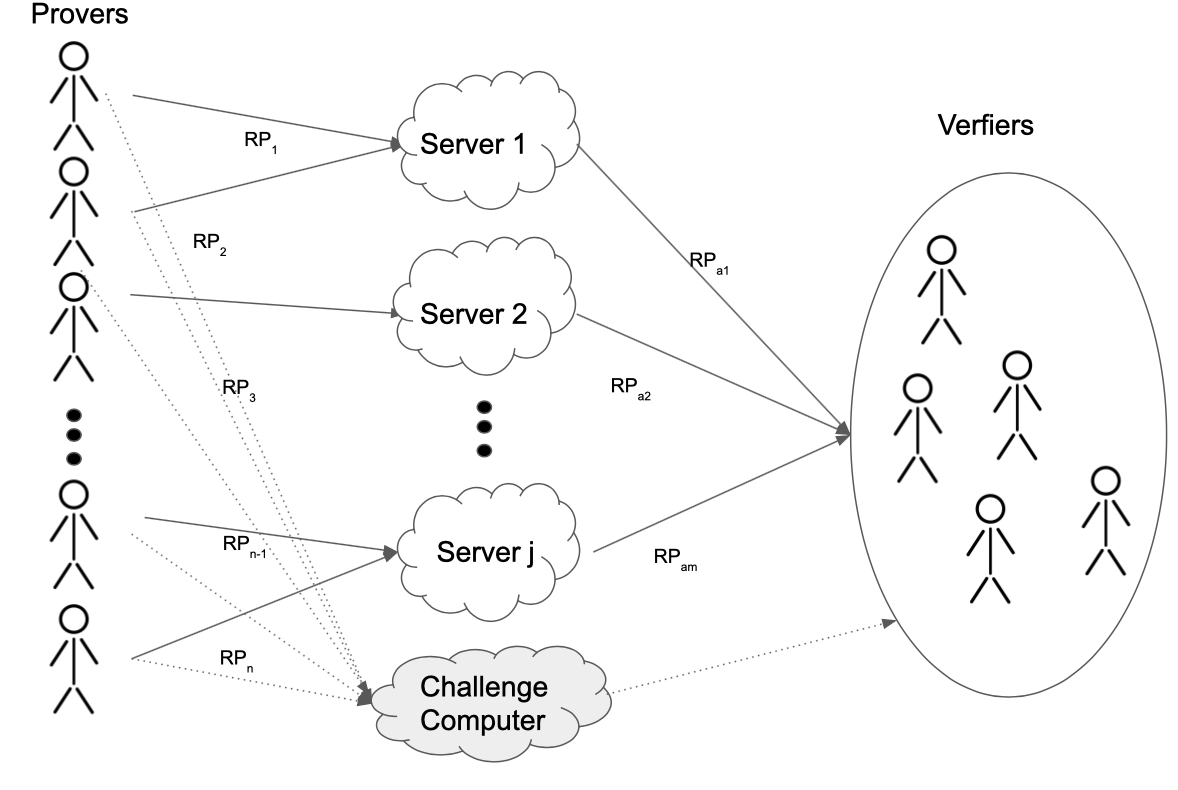
\includegraphics[width=\linewidth]{./figure/workflow_challanger.png}
\end{figure}
To conclude, if the aggregation is not assumed to be performed by a trusted party then due to the characteristics of the VAHSS construction all range proof cannot be aggregated together, instead two or more subsets of the range proofs must be aggregated separately and then all such aggregated range proofs are verified by the verifier. 

The arguments given for the assumptions of the aggregating party and arguments for the aggregated proof satisfying the completeness, soundness and zero knowledge  does not act as formal proofs. therefore all potential attacks on aggregated set membership proof can not be deducted and before using it in practise further security checks need to be performed. 





\subsection*{Aggregating Bulletproofs}
Next lets briefly consider Bulletproofs. The original paper about Bulletproofs \cite{bulletProofs_theory} presents a method to aggregate Bulletproofs such that $n$ parties each having a Pedersen commitment $C_i,\: i=1,...,n$ can generate a single Bulletproof verifying that each commitment hides a secret in an allowed range. This however only works if all parties uses the same challenge $c$ in the proof construction, this is achieved by introducing a dealer. The dealer can be either one of the clients or another party. During the constructions of the proofs when computing the challenges each client sends their proof of to this point to the dealer who aggregates the proofs and computes the challenges based on the aggregated proofs. For example, assume $n$ clients and denote their respective proofs with a subscript $i$, then to compute the challenges $y_i$ in construction \ref{alg:bullet} instead of each client computing $y_i = Hash(A_i,S_i)$, each client sends $A_i,S_i$ to the dealer who adds then homomorphically $A = \prod_{i=1}^n A_i, S = \prod_{i=1}^n S_i$ and the send back the challenge $y =Hash(A,S)$ to be use by all clients. This procedure is repeated for each challenge. The following steps is not describe here instead it is noted that although the Fiat-Shamir heuristic is used to generate the challenges it is interactive since communication between the dealer and the clients is required during the construction of the aggregated range proof. If this procedure was ignored and each client instead computed their own challenges via Fiat-Shamir heuristic and the proof where aggregated after they were fully constructed,  then the challenges would differ between parties and the verification fail. Concluding, it has been seen that the  Bulletproof can be aggregated with the cost on an  interactive construction, however this is not a desirable property for the the server and client verifiable AHSS construction. An further investigation about whether this construction can be modified to be completely non-interactive  has not been done and remains an open question.  

%This concludes that neither of the considered range proofs has be sucessfully fully aggregated aggregated  such that the verifier can perform one single verification instead of one for each client, at least not without some cost. Remark that this conclusion is not final and their may very well exist small or large modifications of the range proof that will allow them to be aggregated and still remaining non-interactive. The investigation of such modification is outside the scope of this paper but the reader is endorsed to explore this possibility. 

\section{Implementation}
To practically investigate the combining of the VAHSS construction \ref{alg:VAHSS-HSS} with a range proof, construction \ref{alg:VAHSS-HSS-RP} is implemented. %is provided written in Golang. 
%Remark that this construction is written without specifying which range proof that is used, and works for all different range proofs that provides a proof for a Pedersen commitment, which is true for all range proof discussed above.
 From the analysis of the range proofs given above it is clear that Bulletproofs is faster than signature-based range proof, however considering the aggregation possibility for signature based range proof these might still be competitive for combination with VAHSS.  All three constructions will hence be used to implement the client and server verifiable additive homomorphic secret sharing construction \ref{alg:VAHSS-HSS-RP}. 

Implementations of Bulletproofs, set membership proofs and signature based range proofs written in Golang (Go) are all available on Github \cite{Git:RP}, implementations of the VAHSS construction \ref{alg:VAHSS-HSS}, written in both python and C++, is available at Github \cite{Git:python_vahss} \cite{Git:C_vahss}.
Because the implementation of the range proofs, set membership proofs and the VAHSS construction is not written in the same programming languages one of the two following modifications needs to be done. The first alternative is to write a wrapper for either the Go code so that it can be interpreted by a C++ (or Python) compiler, or wrap the CC++ (or Python) code such that it can be interpreted by a Golang compiler. The second alternative is to translate either the Go implementations to C++ (or Python) or the other way around. 

The first alternative appears to be a simpler approach hence this is first tested. In 2016 \textit{cgo} was released which enables calling C functions from Go code. 
The Go command \textit{cgo} enables Go packages to call C code. TODO...

This lead to instead test the second alternative, that is translating  the Go implementations to C++ (or Python) or the other way around. Since the VAHSS construction is more straight forward and much shorter than the two range proofs and the set membership proof all together this direction was chosen and Construction \ref{alg:VAHSS-HSS} was translated to Go.

Besides translating the VAHSS implementations to Go a small adjustments of the already existing Go implementations of the range proofs and set membership proof  had to be done to merge with the VAHSS construction. This adjustment are merely to merge the codes and does not change the semantics of the range proofs. What has been  modified is that the randomness used in the Pedersen commitments in the range proof must be chosen such that $R_n = \phi(N)\lceil \frac{\sum_{i=1}^{n-1}R_i}{\phi(N)}\rceil- \sum_{i=1}^{n-1}R_i$, hence is is regarded as input to the proof constructions.The full code for combination of range proofs (or set membership proofs) and VAHSS is available at Git \ref{Git:MyCode}. 

Just as in construction \ref{alg:VAHSS-HSS-RP} the implementation of the code aims to be  general, such that all three concerned range proofs can be used to verify clients honesty and the merge of the range proof to the VAHSS construction is the same for all range proofs. However note that although the construction does not specify which range proof that is used the implementation does due o the choice of underlying group in the set up, the signature-based range proofs and set membership proof uses pairing friendly elliptic curve groups in the implementation which is not the case for Bulletproofs. This leads to minor modifications of the implementation to adapt to range proofs and set membership proofs.

Lets specify what parameters that has been used for the implementation. The number of servers is set to $5$ and the number of clients to $100$.  The range is set to $[18,200]$ for both range proof implementations. This leads to that the parameter $n$ in the Bulletproof construction determining the complexity must be atleast $8$ since $2^8>200$, to keep runtime low it is put equal to eight and for the signature-based range proof, having fixed $u=57$ it is found sufficient to put $l=2$. To make the set membership implementation comparable the size of the set is equal to the length of the range , i.e $|\Phi|=200-18 = 182$.

 For the prototype analysis of the server verifiable AHSS, performed in \cite{VAHSS}, the finite field $\mathds{F}$ used for the secret shares generation is based on a $64$-bit prime number, i.e $\mathds{F}=\mathds{Z}_p$, where $p$ is a $64$-bit prime number,  but in the server and client verifiable AHSS the finite field is formed by a $256$-bit prime number.  The range proofs are based in libsecp256k1 library available in Go-Ethereum and uses elliptic curves and $128$-bit security, to provide this security level the underlying field has to be of size $\sim 256$-bits since the fastest known algorithm to solve elliptic curve discrete logarithm problem (ECDLP) requires $\mathcal{O}(\sqrt{n})$ steps. To use a common underlying field  for the both constructions,  the size of the field for the VAHSS is $256$-bit instead of $64$-bit. The hardware is the same as used above for benchmarking in section \ref{sec:PrototypeAnalysis}. For completeness it is repeated here; the computer used has a $1.6$ GHz Dual-Core Intel Core i$5-5250$U CPU, $8$GB $1600$ MHz DDR3 RAM  and running macOS $10.15$. 




%The size of the underlying range will vary to investigate the impact it has on runtime, both the complexity for the Bulletproofs and signature-based range proof depends on the size of the range unlike the set-membership as discussed above. 

A final remark about the implementation is that its purpose is to test the concept on the above proposed construction and provide runtime evaluations, the code has not been tested enough to be used as secure implementation.

%TODO Describe changes in their code

%bulletproofs, set membership proofs and signature based range proofs to  verify the clients input. in written in Golang. All three mentioned range proofs has previously been implemented in Golang and the code is available on Github at \cite{RP_code}. The server verifiable secret sharing construction has been implemented in python and c++ and is available at Github at \cite{Vahsss_code}. 


%The implementations is done in Golang. Specify all parameters used for the implementation. 
